% !TeX root = ../main.tex
% Add the above to each chapter to make compiling the PDF easier in some editors.

\chapter{Evaluation}\label{chapter:evaluation}
In this chapter we describe the test experiment that was held during the thesis study. The plan for the experiments is described in Section \ref{section:experiment_design}, the description of the actual studies in in the Section \ref{section:experiment_conducting} and the analysis of the data collected during the experiment is in Section \ref{section:experiment_result_analysis}. In Section \ref{section:evaluation} we present the evaluation of the integrated data collection approach according tot the feedback of the participants.\\

%--------------------------------------------------------------------
\section{Experiment design}\label{section:experiment_design}
The goal of the experiment was to conduct a light version of the study that would reflect the actual study on the evaluation of the MaCon approach, integrate surveys and bookmarks that would emulate surveys and bookmarks used for an actual evaluation and, finally, collect the impression about the experiment data collection from the participants.\\

The design of the study depends on the goal of the experiment. Usually the study would require the participants to go through all the development process and create a prototype of a system. Going through all the development process is redundant for the goal of this study. Basically we need the participants to get introduced to the general development approach and make them work with the workbench tool and find out how the data collection influences the work with the tool, how useful it is and how the subjects react to it. It was preferable to show the participants such important aspects of the workbench as modeling and simulation, system decomposition for them to get a wider impression of the application of the tool.\\

Therefore the following format was selected for the experiment. The participants were presented with a finished project with a working model of a simple system. All the requirements were deleted and the task of the participants was to review the prototype of the system presented in the workbench, extract the understanding of the actual system the prototype presented and create requirements for the system that would meet the model.\\

The participants were presented with a system that models a simple conveyor. The system contained one Component - the actuator that performs the movement of the conveyor and one template - the box that was moved by the conveyor. There was one scenario that showed the main behavior of the system - the actuator moved the block from the start point to the end point (see Figure \ref{fig:workbench_1}).\\

\begin{figure}[htb]
 \centering
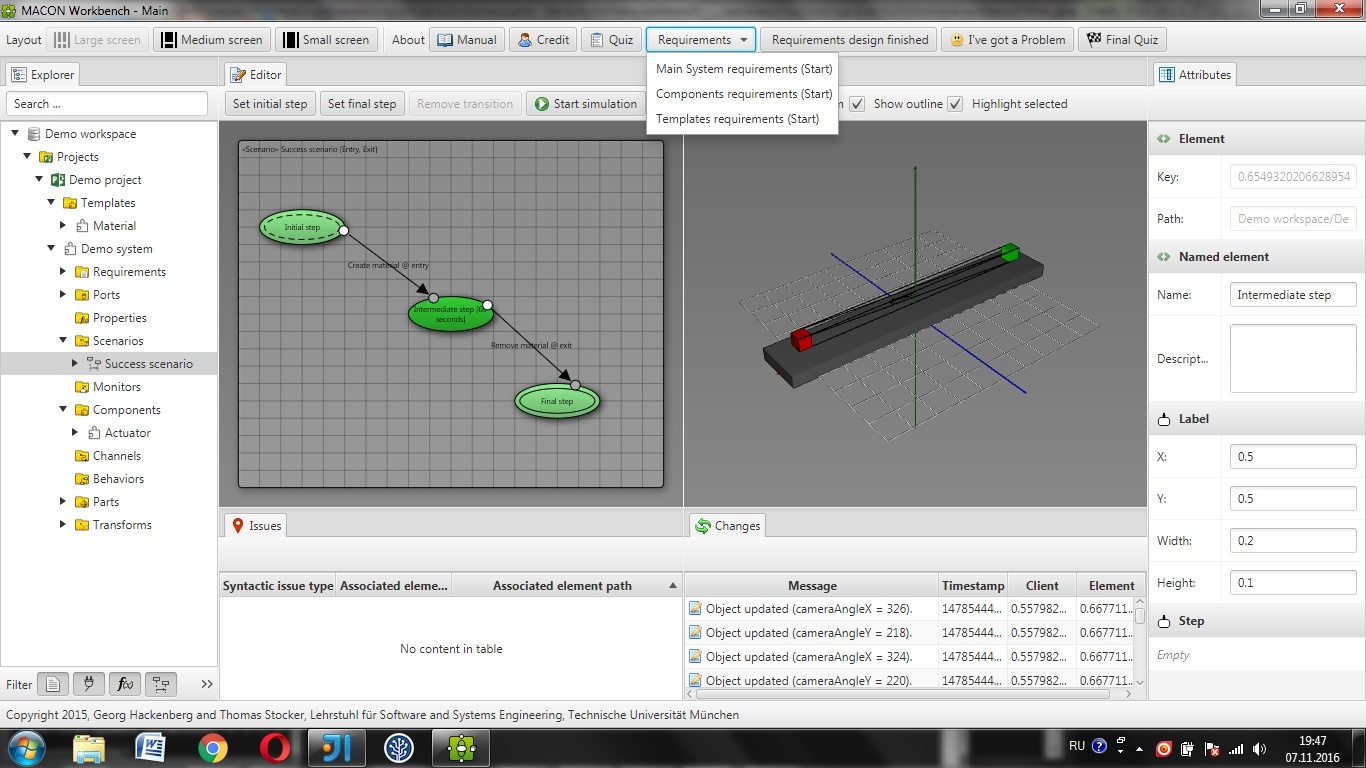
\includegraphics[width=\textwidth]{figures/workbench_1.jpg}
\caption{Conveyor project used during the experiments}
\label{fig:workbench_1}
\end{figure}

The participants were supposed to create requirements of the main system, the template and the component. It was supposed that they will create at least three requirements during the experiment. There were three main activities during the study: Main System Requirements design, Components requirements design and Templates requirements design. There were three time interval Bookmarks for each of them with Surveys about the flow of the corresponding activity (see example on Figure \ref{fig:templates_survey}). The questions included questions about usability, engineering process, position of the activity in the recommended development process and other. The Bookmarks were grouped under the \textit{Requirements} menu. \\

\begin{figure}[htb]
 \centering
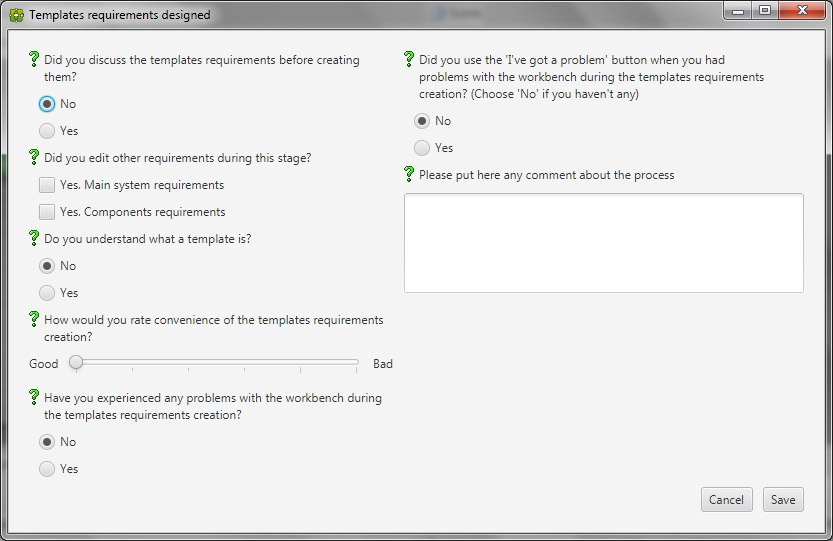
\includegraphics[width=\textwidth]{figures/templates_survey.jpg}
\caption{Templates Requirements design finished Survey}
\label{fig:templates_survey}
\end{figure}

The \textit{Quiz} button to triggered the bookmark that contained a questionnaire about the background of the participant, like experience with mechatronics, age, education, etc. \textit{Requirements design finished} button called the questionnaire with questions about the overall usability of the workbench, naming of the elements, complexity, disadvantages, etc. Button \textit{Final Quiz} called a Survey that had questions about the bookmarks, integrated media files collection, surveys, design of the experiment, etc (see Section \ref{section:evaluation}). Button \textit{I've got a problem} triggered the bookmark and showed a small Survey that offered to select a type of a problem and an area to add details in a free form.\\

There was also a custom trigger configured to be called when the Simulation ends. It showed a Survey window, to collect short feedback about the Simulation.\\

According to the experiment design the participants had a common understanding of the engineering process and the role of the workbench in the process, they worked with different aspects of the tool, including system decomposition into components and templates, simulation to understand the modeling capability of the tool and had an experience in simultaneous object creation and editing, which allowed them to get an opinion about the usability of the workbench.  They also worked with all three types of Bookmarks, so were able to give feedback about them. The design of the experiment didn't require any specific mechanical or electronic engineering knowledge what simplified the process of finding the participants. The experiment was designed to take around 30-40 minutes in total.\\


%--------------------------------------------------------------------
\section{Experiment conducting}\label{section:experiment_conducting}

Initially it was supposed to have multiple experiments to collect data from 20 participants, which is the sufficient number of participant for a quantitative studies according to Nielsen \cite{nielsen}, although the results were very similar, therefore it was decided that 16 participants is enough (see Section \ref{section:evaluation}). Most of the participants were students or recent graduates. The participants had different background (see Figure \ref{fig:background}), but most of them had a background in Informatics (9 participants) or Mechanical Engineering (4 participants). According to the experiment design, the participants were divided into groups of two-three, because otherwise the teams would be too big for the task. There were 7 experiments held: two for a team of three and five for a team of two.\\

\begin{figure}[htb]
 \centering
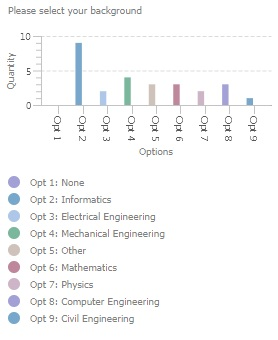
\includegraphics{figures/background.jpg}
\caption{Background of the participants}
\label{fig:background}
\end{figure}

The participants were explained that they are being on an experiment for a Master thesis, introduced to the goal of the experiment and to the general plan of what they will do during the study. They were warned that there would be recording and that the recording would start as soon as they launch the software. Then the researcher explained the participants the general concept of a manufacturing system and the scope of the application of the workbench in manufacturing engineering.\\

The attendants were introduced to the MaCon engineering approach and the workbench, including the concepts of Components and Templates and requirements for those on an example. Then the participants got the detailed description of the task and the plan of the experiment including the recommended sequence of activities to perform the task, that looked as following:
\begin{enumerate}
\item \textit{Quiz}
\item Review of the system: project structure, running simulation etc
\item Discussion of the system 
\item Creation of the requirements
\begin{enumerate}
 \item Main System requirements: discussion and creation of the objects
 \item Components requirements: discussion and creation of the objects
 \item Templates requirements: discussion and creation of the objects
\end{enumerate}
\item \textit{Requirements design finished} survey
\item \textit{Final Quiz}
\end{enumerate}

It was mentioned that the participants are free to change the sequence of the activities and that the button \textit{I've got a problem} can be used at any time to leave any kind of feedback. During the experiment the participants performed the main task following the recommended order of activities and in average created 6 requirements per team, used the bookmark buttons in proper moments, filled the surveys, were generally comfortable with the experiment flow and were rewarded with a cupcake.\\


%--------------------------------------------------------------------
\section{Experiment results analysis}\label{section:experiment_result_analysis}

The results of the experiments didn't show much outcome in the terms of the evaluation of the engineering process and modeling technique, because it wasn't the scope of the study. The participants didn't have enough knowledge about tool-based engineering approaches and experience with manufacturing engineering and the challenge didn't give much understanding about the modeling technique and development process, therefore there couldn't be any valid feedback extracted about engineering process and modeling technique. Moreover, as the case didn't cover the engineering process, but rather one phase - requirements engineering it made no sense to have a retrospective analysis to evaluate the process and the model. Therefore the analysis focused on the usability of the prototyping tool. \\

During the analysis the researcher reviewed the collected data. It's possible to draw an understanding of the general impression of the workbench as well as knowledge of what the participants think should be changed to improve the workbench. For example, on the Figure \ref{fig:results1} you can see that the majority of the respondents think the workbench needs changes to be used in the industry, 6 respondents find the navigation complicated and 4 respondents imply that the UI is inconvenient.\\ 

\begin{figure}[htb]
 \centering
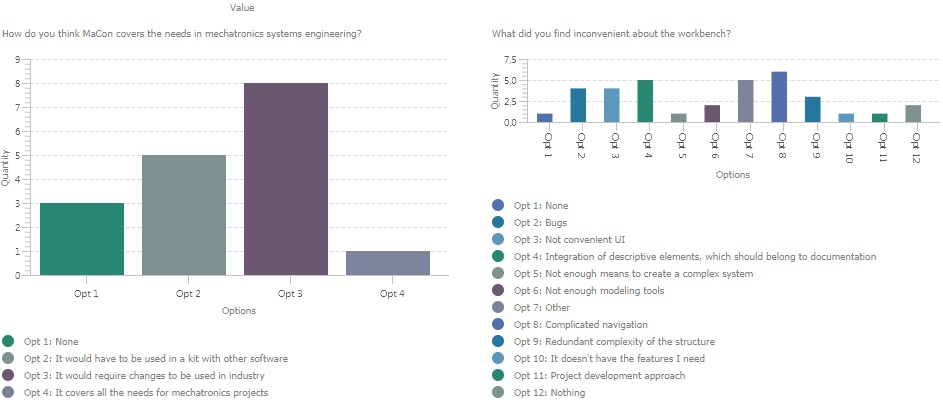
\includegraphics[width=\textwidth]{figures/results1.jpg}
\caption{Feedback about the workbench}
\label{fig:results1}
\end{figure}

Therefore the researcher investigated the free form text answers to find which part of the navigation and usability of the UI could be improved. From the analysis of the text question the researcher can find out that participants have problems with renaming the folder when a child object is created. The users expect the newly created object to be selected for editing immediately after creation, three respondents specified that they would like to edit the name of the object in the explorer tab or the editor tab.\\

Visualization of the Likert Scale answers in the form of one-dimensional bubble chart is intuitive and easy to understand without the close look on the answers. For example, Figure \ref{fig:convenience} shows how the answers about the convenience of the requirements creation change through the flow of the activities. After the first activity most of the participants rated the convenience as Good, after the end of the second activity the answers shifted closer to the negative answers and by the end of the third activity the majority of the attendants rated the convenience as 3/6, which is still in the positive part of the scale, but the tendency shows that the participants were finding the workbench more inconvenient during the experiment.\\     

\begin{figure}[htb]
 \centering
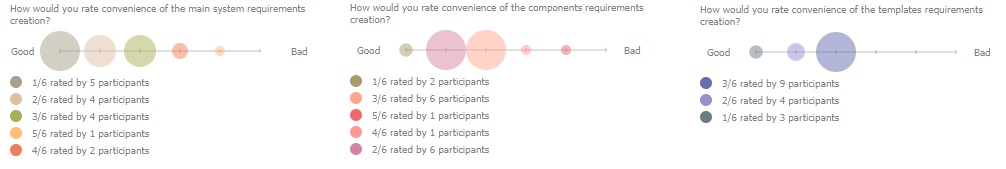
\includegraphics[width=\textwidth]{figures/convenience.jpg}
\caption{Feedback about the convenience of requirements creation}
\label{fig:convenience}
\end{figure}

This tendency might be the results of the participants getting to know the tool better or because of the frustration caused by filling Surveys. Figure \ref{fig:surveys_time} shows that in general the participants were filling the surveys more time than they expected to.\\

\begin{figure}[htb]
 \centering
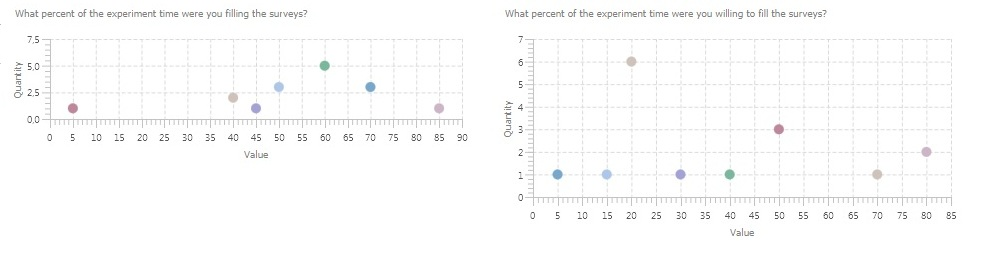
\includegraphics[width=\textwidth]{figures/surveys_time.jpg}
\caption{Feedback about the percentage of time spent on surveys}
\label{fig:surveys_time}
\end{figure}




%--------------------------------------------------------------------
\section{Evaluation of integrated data collection} \label{section:evaluation}

The feedback about the integrated data collection is presented in the Figure \ref{fig:final_qiz}. As you can see, all the participant found the integrated surveys useful and 11 out of 16 respondents found integrated media files collection comfortable as it is. The majority of the participants marked that they enjoyed the integrated surveys, 12 participants marked the integrated surveys at the most preferable way to collect data comparing to paper surveys or online tools like Google forms etc. Only one participant found the integrated questionnaires distracting.\\

\begin{figure}[htb]
 \centering
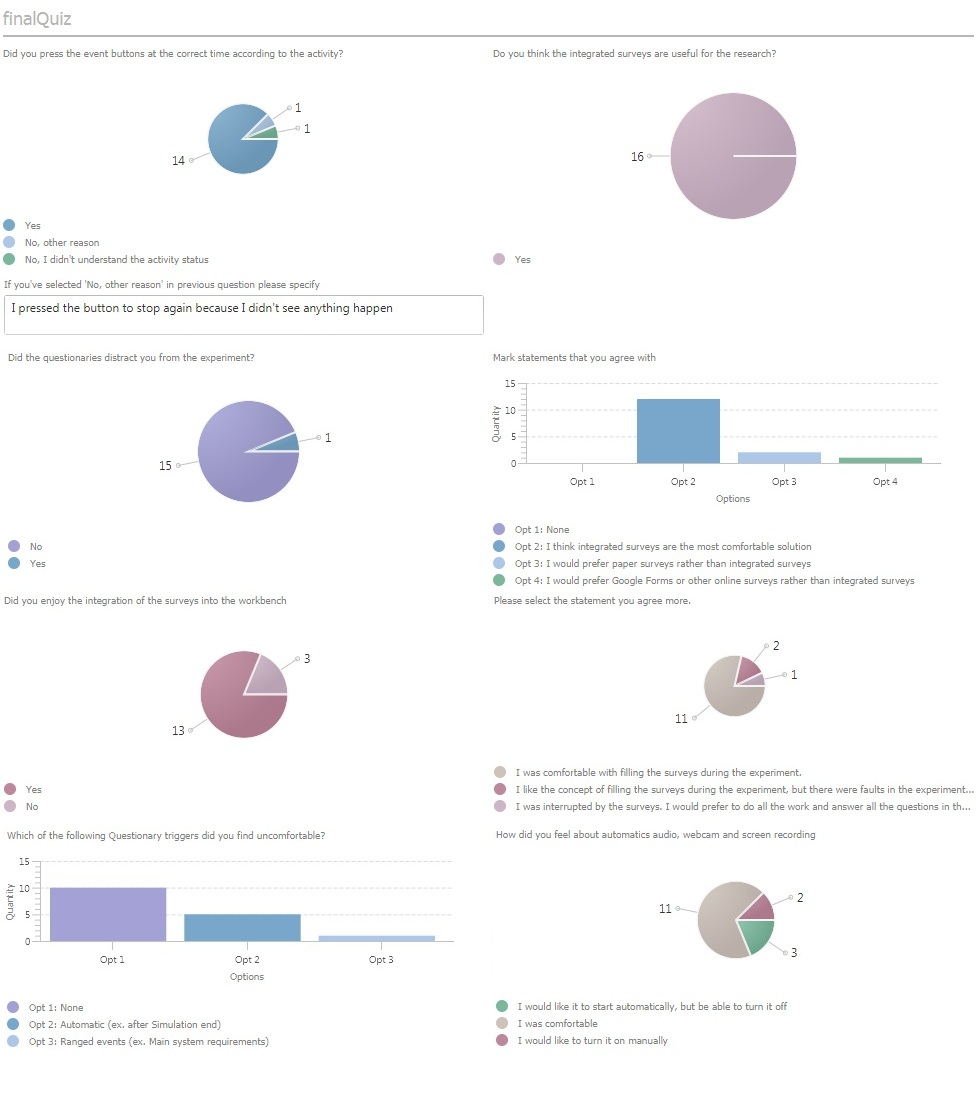
\includegraphics[width=\textwidth]{figures/final_qiz.jpg}
\caption{Feedback about the integrated data collection}
\label{fig:final_qiz}
\end{figure}

Concerning the types of the bookmarks, 14 of the residents didn't have any problems with the time intervals. One of the participants complained that the change of the name of the menu item isn't noticeable enough and he didn't realize the state change. Possible improvement would be to substitute labels \textit{Start} and \textit{Stop} with graphical icons. Five Participants stated that automatic trigger made them feel uncomfortable. That might have been caused by the fact that the trigger was configured to happen every time the simulation ended, which might be too often, although in average the participants ran the simulation twice.\\

Observing the experiment left the impression that the participants were comfortable with the integrated data collection and stayed focused on the work within the workbench. The instructions were clear and the integrated data collection didn't raise any additional questions or problems. According to the experiment goal explanation, the attendants treated the bookmarks and questionnaires as an important part of the study and were attentive on marking the intervals and answers in the surveys.\\ 


